\documentclass[12pt, letterpaper]{article}
\usepackage[utf8]{inputenc}
\usepackage[italian]{babel}
\usepackage[T1]{fontenc}
\usepackage{graphicx}
\graphicspath{}
\usepackage{listings}
\usepackage{svg}
\usepackage{pdfpages}

\title{Progetto per il corso di Progetto Automatico di Sistemi Digitali}
\author{Filippo Landi}

\begin{document}
\maketitle

\begin{abstract}
Il mio progetto per il corso di \textit{Progetto Automatico di Sistemi Digitali} (\textit{PASD} in breve) consiste nello studio statistico del comportamento di un circuito \textit{multiply and accumulate} (o \textit{mac} in breve) in presenza di alcuni difetti di produzione.
\end{abstract}

\section{Introduzione al progetto}

Il progetto riguarda il collaudo dei sistemi digitali, un argomento trattato ampiamente nel corso.

Al fine di simulare i guasti del circuito userò \textit{HOPE}: un simulatore di guasto per circuiti sincroni e sequenziali proposto durante il corso.

HOPE è stato sviluppato dall'università VirginiaTech ed è rilasciato per uso universitario o di ricerca, per averne una copia bisogna entrare in contatto con l'università di VirginiaTech: io non lo condividerò in questo progetto.

HOPE legge i circuiti attraverso delle descrizioni della rete (dette anche \textit{netlist}) in formato \textit{.bench}, infatti il primo punto del progetto sarà l'implementazione del circuito in questo formato.

Ho usato \textit{Python} per diversi passaggi del progetto: 
\begin{itemize}
\item Non è un linguaggio efficiente come ad esempio il linguaggio C, però mette a disposizione funzioni built-in per la manipolazione di stringhe che si sono rivelate molto utili.
\item Ci sono molte librerie interessanti per Python come la libreria \textit{matplotlib} che mi ha permesso in maniera comoda di realizzare dei grafici dei dati raccolti.
\end{itemize}

I prerequisiti software quindi sono:
\begin{itemize} 
\item \textit{Python} in versione superiore alla 3.6.
\item Il software \textit{HOPE}.
\item La libreria \textit{matplotlib} (con le varie dipendenze).
\end{itemize}

L'esposizione del progetto seguirà questo flusso: 
\begin{enumerate}
\item Vedremo l'implementazione del circuito in termini di porte logiche.
\item Vedremo la sua implementazione in un file .bench attraverso lo script \textit{mac\_generator.py}.
\item Vedremo come usare HOPE per i nostri scopi.
\item Calcoleremo delle statistiche attraverso lo script \textit{getstats.py}.
\item Infine commenteremo i risultati con alcuni grafici.
\end{enumerate}

Ho inoltre modificato gli script per renderli compatibili con la versione 2.7 di Python, tranne per la costruzione automatica dei grafici.

\section{Circuito multiply and accumulate}

Inizialmente mi è stato richiesto di realizzare un circuito multiply and accumulate (mac) a 8 bit.

Un mac è composto da un moltiplicatore con un sommatore in cascata e un registro che retroaziona le uscite in modo da accumulare i risultati.

Riporto la documentazione che mi è stata inviata dal professore che illustra gli schemi di un mac a 4 bit.

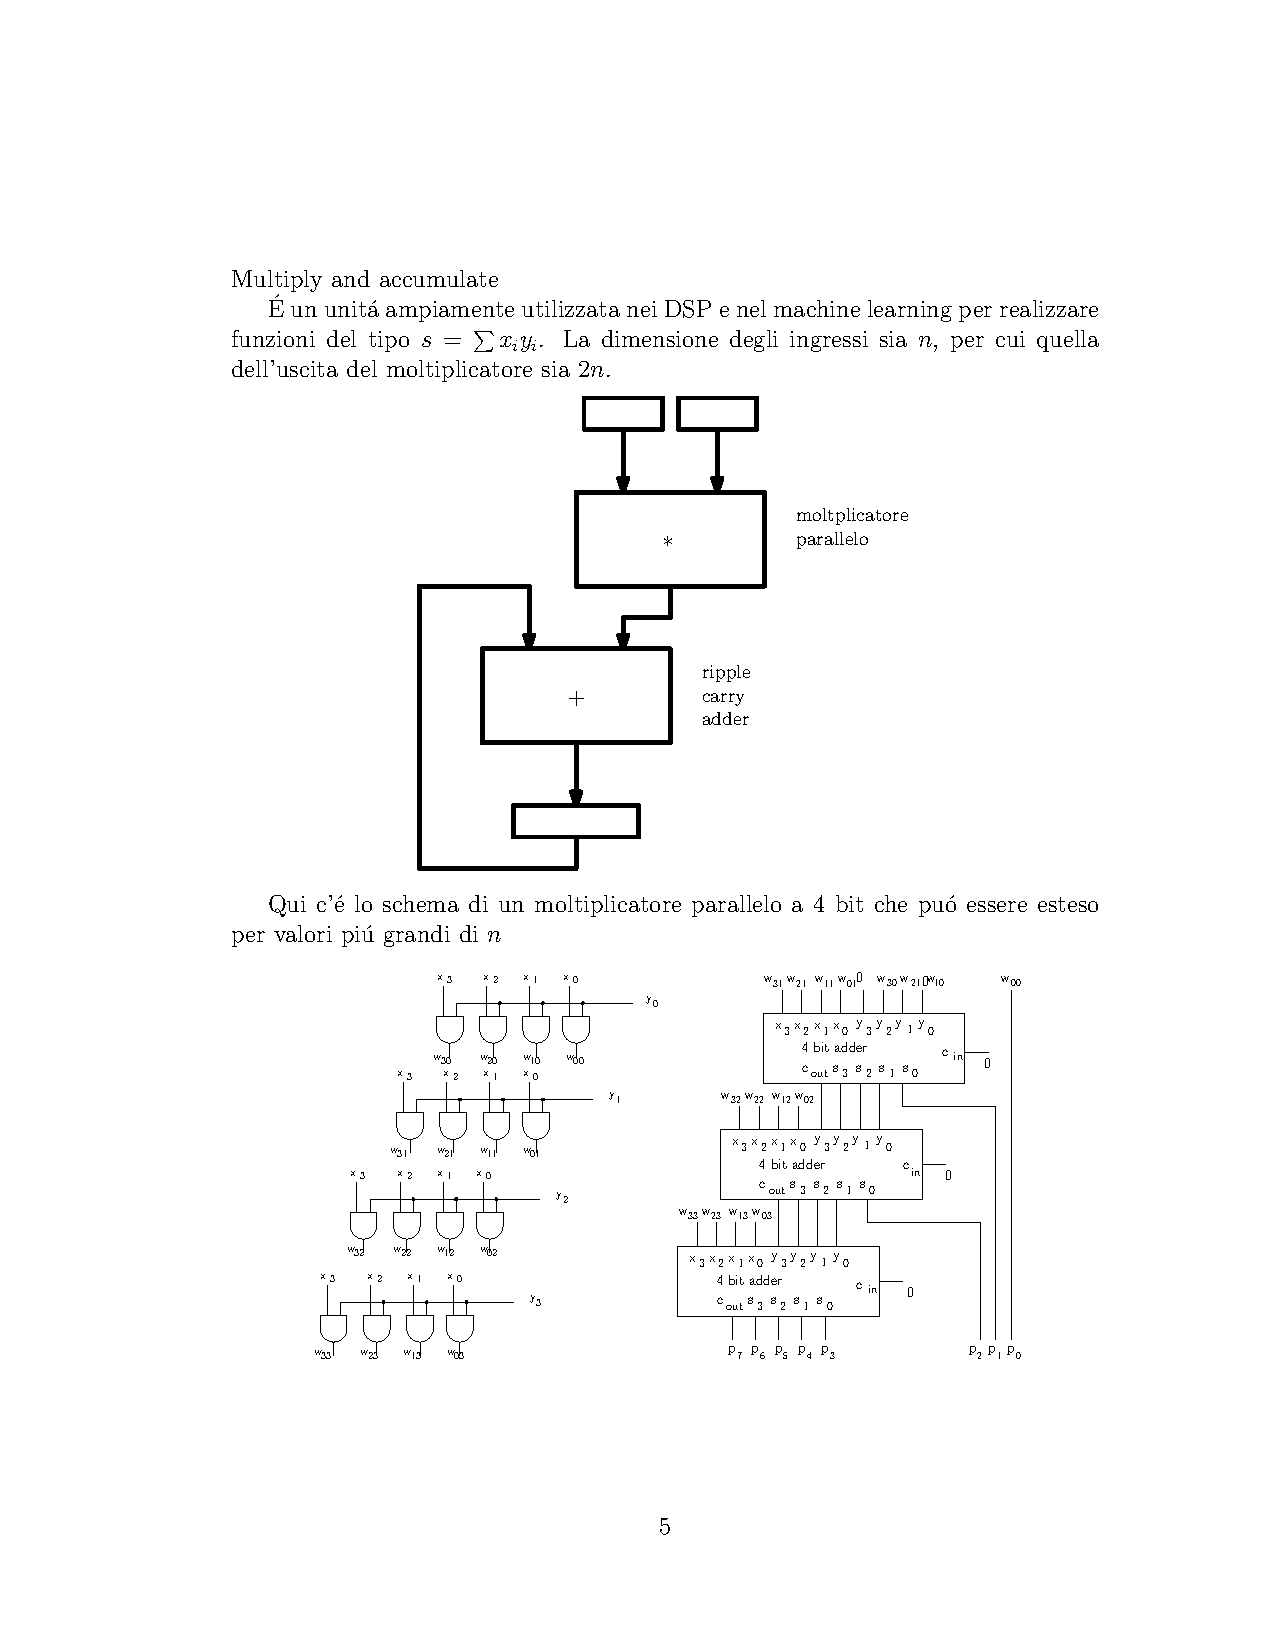
\includepdf[pages=-,frame=true,noautoscale,scale=0.9]{prova5.pdf}

\newpage
\subsection{Moltiplicatore}
La struttura del moltiplicatore è ben illustrata nella documentazione:

\begin{itemize}
  \item Ogni segnale X è messo in AND con ogni Y, generando i segnali W.
  \item I segnali W vengono usati da degli adder strutturati su più livelli: si può notare che il numero di livelli è \textit{n-1} in quanto al primo livello vengono usati WX1 e WX0, poi i rimanenti WXY nei livelli successivi.
\end{itemize}

\subsection{Sommatore}
È un \textit{ripple carry adder} (\textit{rca} in breve) con dimensione degli ingressi 2n: un ingresso è dato dall'uscita del moltiplicatore mentre l'altro è dato dalle uscite stesse del sommatore retroazionate attraverso dei flip-flop tipo D (circuito già integrato in HOPE).

\subsubsection{Ripple Carry Adder}

Usiamo dei circuiti ripple carry adder sia per la cascata di adder del moltiplicatore sia, come già detto, per il sommatore.

Questi circuiti nella precedente documentazione erano illustrati a livello \textit{register transfer level} (\textit{RTL}) per ragioni di chiarezza: per l'implementazione ci serve vedere come sono fatti a livello di porte logiche.

Gli rca sono formati da una serie di adder opportunamente collegati: gli adder sono half-adder o full-adder a seconda del peso del bit.

\begin{figure}
\centering
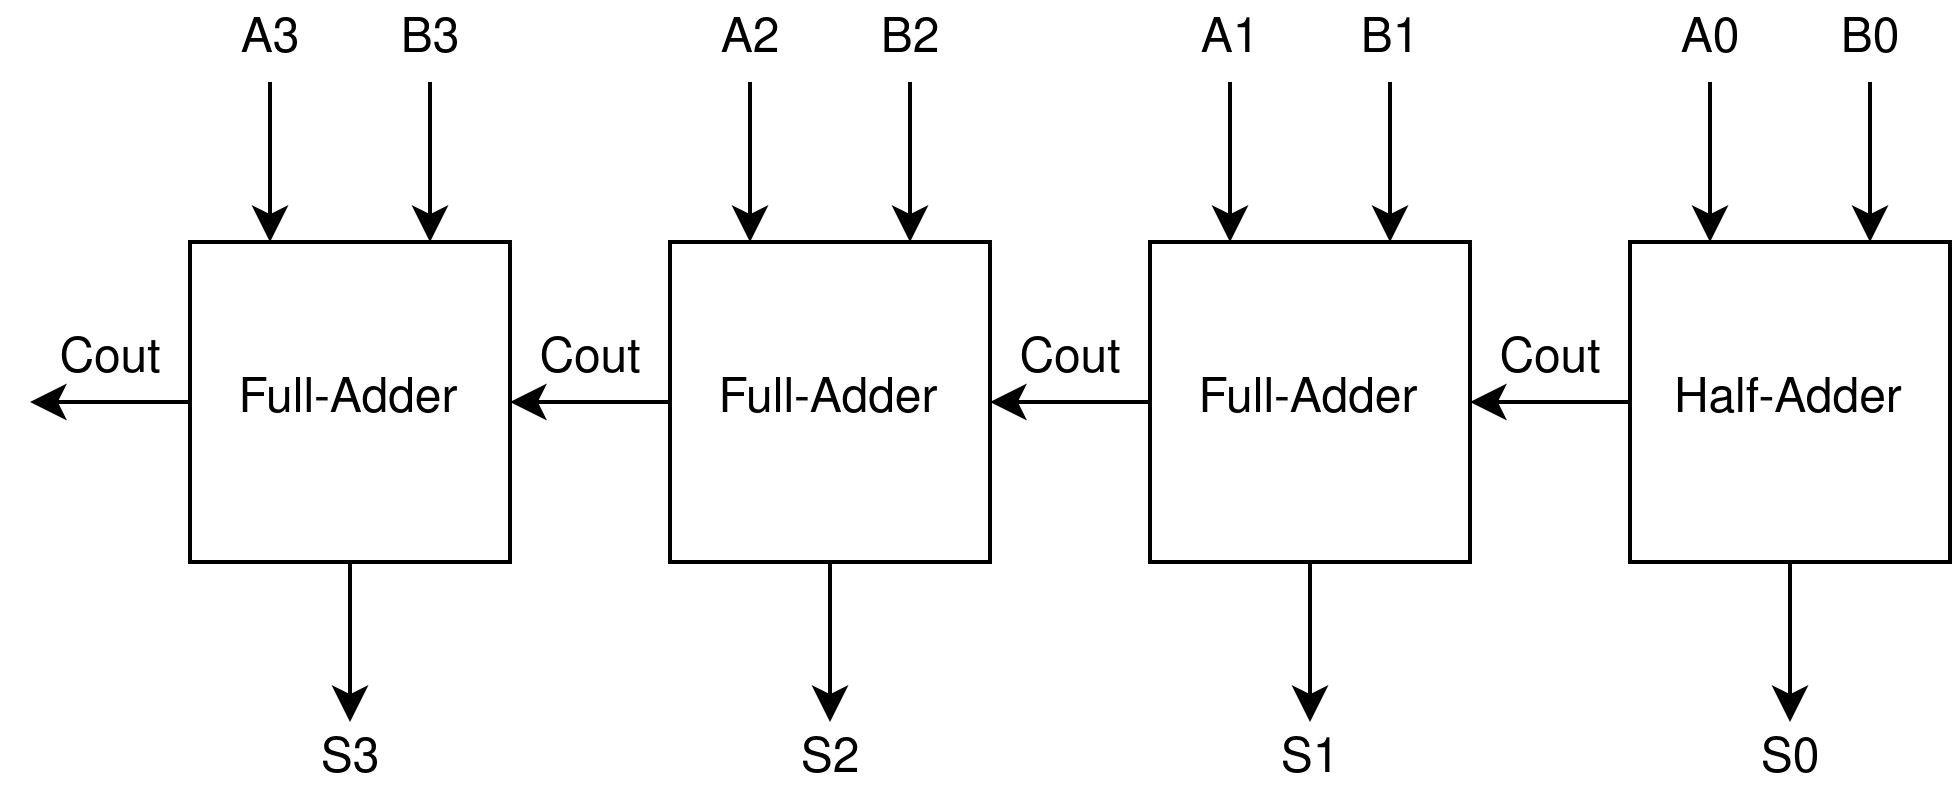
\includegraphics[width=\textwidth]{ripple_carry_adder}
\caption{Schema del ripple carry adder.}
\label{rca}
\end{figure}

\begin{figure}
\centering

\includegraphics{half_adder}
\caption{Schema dell'half-adder.}
\end{figure}

\begin{figure}
\centering
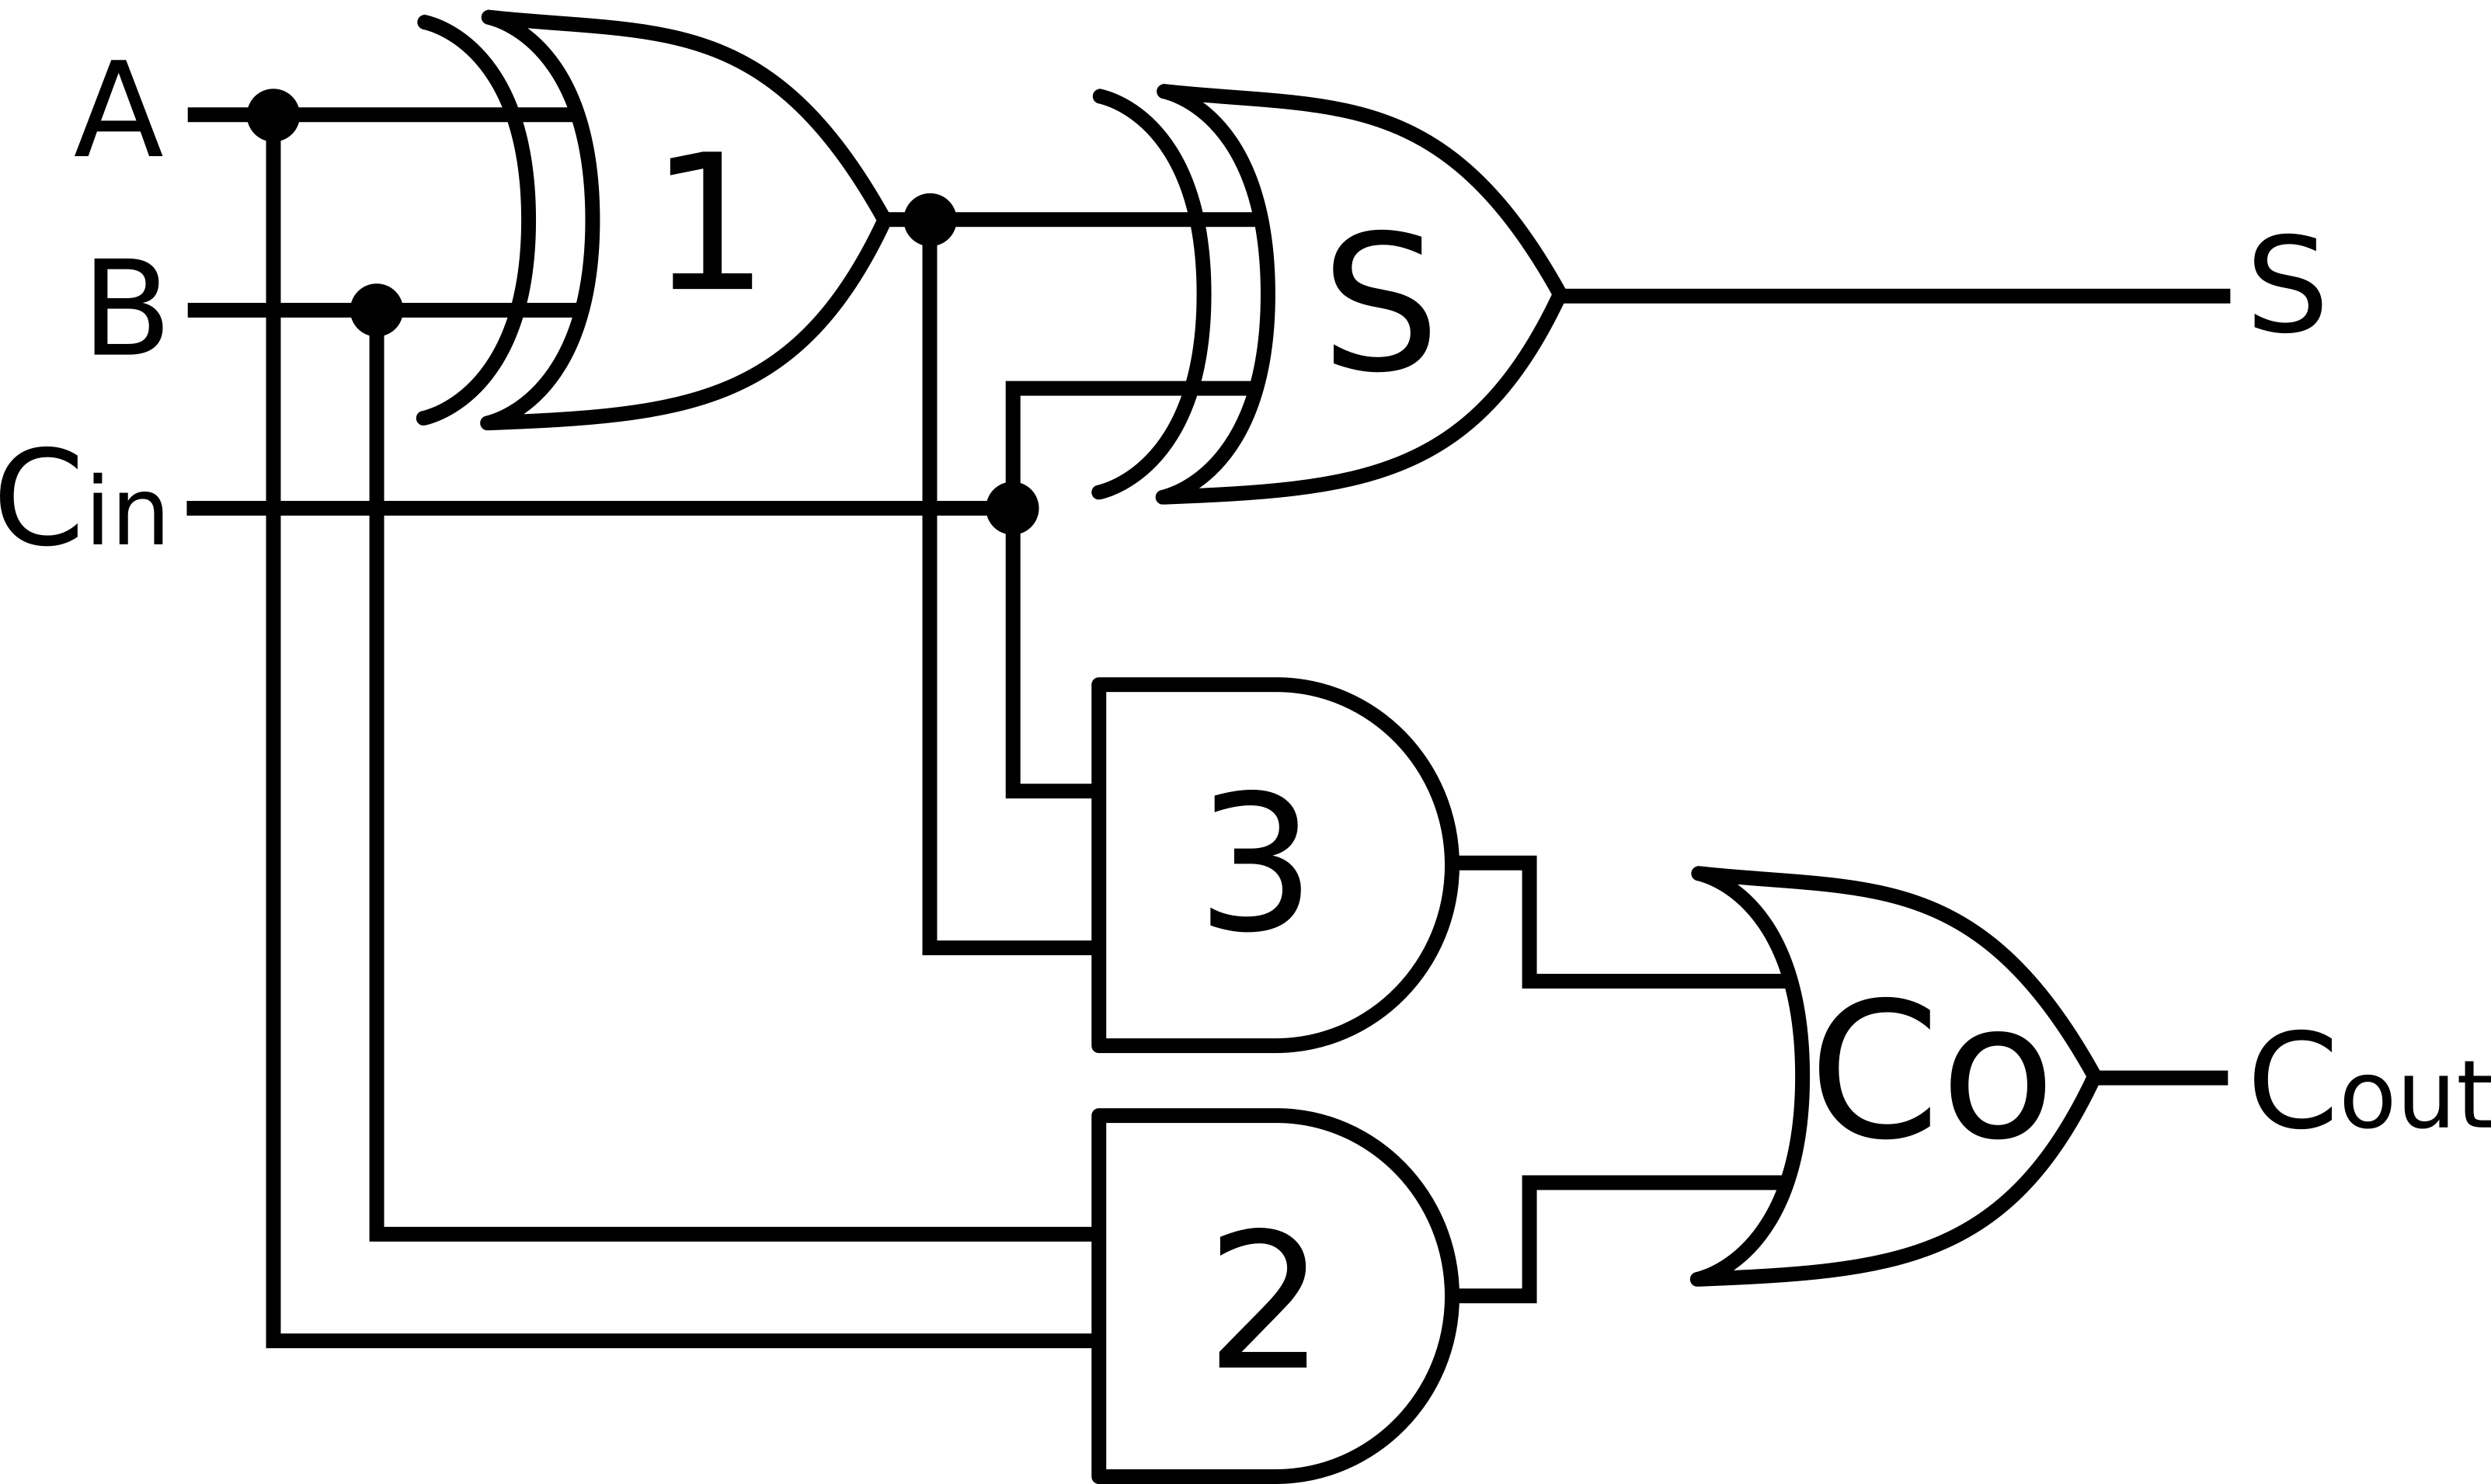
\includegraphics[width=8cm]{full_adder}
\caption{Schema del full-adder.}
\end{figure}

Gli schemi dei circuiti sono riportati alla pagina \pageref{rca}.

\section{Script mac\_generator.py}

La stesura manuale del file .bench del mac ad 8 bit non mi sembrava un approccio furbo vista l'architettura piuttosto complessa da rappresentare. Probabilmente proseguire con tale metologia avrebbe portato a vari errori: sia banalmente di battitura, sia dovuti alla complessità e quindi errori nel collegamento dei vari segnali. Per questo ho pensato ad una metodologia stile \textit{divide et impera}.

In partenza ho scritto alcuni circuiti di prova per esplorare l'implementazione dei vari adder e la prima parte del moltiplicatore.
Li trovate nella cartella \textit{circuti\_prova}: non sono fondamentali per il progetto però possono aiutare alla comprensione della metodologia usata.

Appurata la struttura dei circuiti base, ho creato uno script monolitico \textit{mac\_generator.py} che attraverso alcuni cicli e condizioni li collega in maniera consistente con gli schemi a mia disposizione.
Questo script permette di generare mac con dimensione arbitraria degli ingressi da passare come argomento.
Ad esempio per generare un mac 8 bit si può scrivere da terminale questo comando Python: 

\begin{lstlisting}
python3 mac_generator.py 8  
\end{lstlisting}

Il passo successivo sarebbe un approccio più modulare, che otterrebbe lo stesso risultato chiamando sottofunzioni per la varie parti del circuito: per i miei scopi uno script monolitico è più che sufficiente quindi mi fermo a questa versione.

Il codice è ampiamente commentato quindi consiglio di leggerlo per comprenderne il funzionamento.

L'unico punto che potrebbe essere difficoltoso è la comprensione dei vari segnali: proprio per questo un approccio manuale a mio avviso non sarebbe stato efficiente.

Descrivo quindi la struttura dei vari segnali, sperando che sia di aiuto:

\begin{itemize}

\item Gli input sono facilmente individuabili e sono X e Y seguiti dal rispettivo peso del bit, es. X0,Y0,X1,Y1 etc.
\item I segnali W ottenuti dagli AND di X e Y sono scritti come "W\_XnYn" (n indica il peso del bit), es. W\_X0Y0.
\item I ripple carry adder contengono half-adder e full-adder:

\begin{itemize}

\item Gli half-adder, come dagli schemi, hanno uscita S e Co (il carry out) e sono usati in generale (con qualche eccezione) per il bit di minor peso (bit 0):
\begin{itemize}
\item Nel moltiplicatore gli rca sono strutturati in livelli:
\begin{itemize}
\item SL0D0 indica l'uscita dell'half-adder al livello (L) 0 del bit di peso (D) 0.
\item CoL0D0 indica il carry out dell'half-adder al livello (L) 0 del bit di peso (D) 0, questo carry out sarà il carry in del full-adder successivo.
\end{itemize}
\item Nel sommatore invece non ci sono più i livelli:
\begin{itemize} 
\item S0 indica l'uscita dell'half-adder per il bit di peso 0.
\item C0 il suo carry out.
\end{itemize}
\end{itemize}

\item I full-adder, come dagli schemi, hanno uscita S e Co con l'aggiunta rispetto gli half-adder dei segnali interni 1,2,3:
\begin{itemize}
\item Nel moltiplicatore gli rca sono strutturati in livelli: 
\begin{itemize}
\item SL0D1 indica l'uscita del full-adder al livello (L) 0 del bit di peso (D) 1
\item lo stesso full-adder avrà CoL0D1, 1L0D1, 2L0D1 e 3L0D1 (carry out e segnali interni).
\end{itemize}
\item Nel sommatore invece non ci sono più i livelli: 
\begin{itemize}
\item S1 indica l'uscita del full-adder per il bit di peso 1
\item Lo stesso full-adder avrà Co1, 11, 21 e 31 (carry out e segnali interni) sempre legati al primo bit.
\end{itemize}
\end{itemize}
\end{itemize}
\end{itemize}

Probabilmente i segnali interni dei full-adder sono quelli che creano maggiore confusione nella lettura: nella mia prima analisi li avevo assegnati numerici e li ho mantenuti così, in caso basta cambiarli con una qualche lettera non assegnata.

\subsection{Versione compatibile con Python 2.7}

Lo script mac\_generator.py funziona con Python 3.8.10 e dovrebbe funzionare con ogni versione superiore alla 3.6.

Ho realizzato una versione compatibile con Python 2.7 nella cartella \textit{python2.7}, sotto il nome di \textit{mac\_generator\_python2.py}: le modifiche non comportano differenze nei file di output.

Se interessa, a livello di sorgenti ci sono state queste modifiche:
\begin{itemize}
\item Python 3.6 aveva introdotto le cosidette "f-strings" molto più comode della metodologia precedente per formattare le stringhe: Python 2.7 ovviamente usa la vecchia formattazione quindi ho dovuto sostituire le f-strings con stringhe formattate con .format().
\item Python 2 suppone che tutti i caratteri siano ascii e quindi se trova lettere accentate da' errore quindi ho forzato l'encoding utf-8 con un "commento magico" nella prima riga di codice.
\item La concatenzione delle stringhe avviene in maniera diversa tra le due versioni per le differenze dovute alla formattazione: con il nuovo metodo le stringhe si concatenano automaticamente, con il vecchio bisogna aggiungere un "+".
\end{itemize}

\section{Testing del circuito con HOPE}

Ottenuto il file .bench utilizzando lo script precedente possiamo passare ad usare HOPE.

Spostandosi nella cartella di installazione di HOPE si può aprire la guida utente scrivendo a terminale:
\begin{lstlisting}
./hope -h g
\end{lstlisting}

Per l'analisi dei nostri circuiti in particolare useremo questo comando: 

\begin{lstlisting}
./hope -F fn -r n -0 -N -s m mac_{bit}.bench
\end{lstlisting}

Per spiegare il comando riporto una mia traduzione della documentazione di HOPE sui vari argomenti:

\begin{itemize}
\item "-F fn": Vengono riportate nel file fn le uscite del circuito buono e difettoso per ogni errore. Con questa opzione, l'euristica di fault dropping di HOPE non viene eseguita, vale a dire che tutti i guasti vengono iniettati e simulati in parallelo.(default: l'uscita del circuito difettoso non viene segnalata.) 

NDR: Le linee dove il guasto viene rivelato hanno un asterisco.

\item "-r n": (Modalità a pattern random)
I pattern di test sono generati in maniera random. La simulazione di guasto termina se se tutti i guasti sono stati rivelato oppure se sono stati applicati n pattern. (default: -r 224)

\item "-0": tutti i flip-flop sono settati inizialmente al livello logico 0

\item "-N": Modalità diagnostica. Il fault dropping non è eseguito. Quindi, tutti i guasti sono simulati per ogni pattern di test. (default: i guasti rivelati durante la simulazione di guasto vengono tolti dalla lista dei guasti.)

\item "-s m": Il seme iniziale del generatore casuale di numeri è impostato da m.
Se m=0, il seme casuale è generato usando l'orario del computer. (default: -s 0)

\end{itemize}

In conclusione facciamo questo: avendo dei flip-flop li settiamo a 0 ed eseguiamo la simulazione di guasto con m vettori di test, disabilitando il fault dropping, salvando il risultato in un file con tutti i vari guasti e fissando un seme per rendere i test ripetibili.

Vedremo degli esempi nel capitolo di analisi dei circuiti.

\section{Script getstats.py}

Ho realizzato lo script \textit{gestats.py} per analizzare il file generato da HOPE, basta passarlo come argomento:

\begin{lstlisting}
python3 getstats.py file_hope
\end{lstlisting}

Anche in questo caso il codice è ampiamente commentato e consiglio di leggerlo per comprenderne il funzionamento. 

In breve questo programma esegue questo algoritmo: 

\begin{enumerate}
\item Setta dei contatori a 0 per i guasti rivelati e i guasti iniettati, apre il file e con un ciclo lo legge riga per riga:
\item Se individua la parola "test" in una riga:

\begin{enumerate}
\item Se il contatore di guasti iniettati è diverso da 0, vuol dire che è terminato il test precedente quindi:
\begin{itemize}
\item Calcolo la probabilità di errore in uscita, data dalla divisione tra i guasti rivelati e i guasti iniettati.
\item Azzero i contatori e continuo.
\end{itemize}
\item Sono all'inizio di un nuovo test: da questa riga posso ricavare i vettori di ingresso e l'uscita attuale (e corretta) del circuito.
\begin{itemize}
\item Ogni riga successiva ho l'iniezione di un guasto nel circuito, quindi aumento di 1 il contatore dei guasti iniettati. Se inoltre la riga contiene un asterisco significa che ho un guasto rivelato in uscita e quindi aumento di 1 anche il contatore dei guasti rivelati.
\end{itemize}
\end{enumerate}

\item Quando esco dal ciclo calcolo le statistiche per l'ultimo test e creo un grafico a barre con matplotlib che mostra la probabilità di errore per ogni test.
\end{enumerate}

Per salvare l'output del programma si può ridirigere l'output da terminale a un file a piacimento: es. "getvectors.py mac > output\_mac".
Ridirigere l'output inoltre fa risparmiare molto tempo di esecuzione perché appunto evita l'output a terminale che è piuttosto lento. 

Il programma inoltre salva i vari vettori in file di testo sotto forma di array "vectors\_mac", questo è un semplice dump, probabilmente non di grande utilità: ogni array ha gli ingressi, l'uscita corretta e le varie uscite con guasti iniettati.

\subsection{Script compatibile per Python 2.7}

Ho reso lo script compatibile con Python 2.7 tranne per la creazione dei grafici con matplotlib: mi dava problemi probabilmente per una questione di ambiente poiché si è installato per la mia versione di Python (3.8.10) quindi bisognerebbe provare con degli ambienti virtuali, ma non mi sono addentrato in questo problema.

\section{Analisi dei circuiti mac}

In conclusione vediamo i grafici generati e facciamo qualche commento.

Mi è stato richiesto di analizzare questi dati per i circuiti a 4, 8 e 16 bit.

\subsection{Analisi del mac 4 bit}

Riporto per completezza tutta la procedura:

\begin{enumerate}
\item Creiamo il file \textit{mac\_4.bench}.
\begin{lstlisting}
python3 mac_generator.py 4
\end{lstlisting}
\item Copiamo il file nella cartella di \textit{HOPE} e lanciamo il comando:
\begin{lstlisting}
./hope -F mac_4_t16 -r 16 -0 -N -s 1 mac_4.bench
\end{lstlisting}
N.B.: qui stiamo testando il circuito con un pattern di 16 vettori, useremo un seed di 1 per tutti i test successivi.
\item Copiamo il file \textit{mac\_4\_t16} nella cartella con i gli script Python e lanciamo il comando:
\begin{lstlisting}
python3 getstats.py mac_4_t16
\end{lstlisting}
\end{enumerate}

Questo è il grafico risultate:

\includesvg[width=0.8\columnwidth]{mac_4_t16_stats.svg}

Ripetendo lo stesso procedimento con 32 vettori di test abbiamo questo grafico:

\includesvg[width=0.8\columnwidth]{mac_4_t32_stats.svg}

Ripetendo lo stesso procedimento con 64 vettori di test abbiamo questo grafico:

\includesvg[width=0.8\columnwidth]{mac_4_t64_stats.svg}

Notiamo quindi che raggiunti i 20 test, la probabilità di errore in uscita rimane intorno al 85\% e non cresce più.

Passiamo al circuito a 8 bit mantenendo 64 vettori di test.

\subsection{Analisi del mac 8 bit}

Il procedimento è sempre lo stesso, lo riporto nuovamente per completezza:

\begin{enumerate}
\item Creiamo il file \textit{mac\_8.bench}.
\begin{lstlisting}
python3 mac_generator.py 8
\end{lstlisting}
\item Copiamo il file nella cartella di \textit{HOPE} e lanciamo il comando:
\begin{lstlisting}
./hope -F mac_8_t64 -r 64 -0 -N -s 1 mac_8.bench
\end{lstlisting}
\item Copiamo il file \textit{mac\_8\_t64} nella cartella con i gli script Python e lanciamo il comando:
\begin{lstlisting}
python3 getstats.py mac_8_t64
\end{lstlisting}
\end{enumerate}

Il grafico risultante è questo:

\includesvg[width=0.8\columnwidth]{mac_8_t64_stats.svg}

Abbiamo anche qui un comportamento simile a quello visto prima: indicativamente a 30 vettori la probabilità di errore va in saturazione.

\subsection{Analisi del mac 16 bit}
Vediamo il grafico per il circuito a 16 bit con 64 vettori di test:

\includesvg[width=0.8\columnwidth]{mac_16_t64_stats.svg}

Per curiosità vediamo anche il grafico con 128 vettori di test.

\includesvg[width=0.8\columnwidth]{mac_16_t128_stats.svg}

Notiamo un comportamento simile a quello dei circuiti precedenti: intorno al cinquantesimo vettore la probabilità di errore in uscita arriva al 95\% e non aumenta ulteriormente con i vettori successivi.

\subsection{Ulteriori analisi}

Ho provato la stessa procedura con mac a 32 e 64 bit ma HOPE con l'opzione -F da' un errore di segmentazione: i circuiti sono testabili normalmente ma per qualche motivo non riesce a salvare il file di tale opzione.

\subsection{Analisi conclusiva}

Abbiamo quindi osservato un comportamento particolare: la probabilità di errore parte da un valore basso e poi all'aumentare dei vettori di test satura intorno ad una certa percentuale e continuerà ad oscillare intorno ad essa.

Questo effetto è dovuto a fenomeni sequenziali dovuti al registro.

Per testare questo ho creato un circuito \textit{mac\_4\_noreg} partendo da un mac 4 bit, dove ho eliminato il registro (che quindi ora non accumulerà più) e ho reso accessibile il secondo ingresso del sommatore.

Ripetendo quanto fatto nei circuiti precedenti (eliminando l'opzione -0 che qui non serve) si ottiene questo grafico con un pattern di 64 vettori:

\includesvg[width=0.8\columnwidth]{mac_4_noreg_t64_stats.svg}

Come si può vedere qui non notiamo l'andamento visto precedentemente.

Ho realizzato poi un semplice accumulatore ad 8 bit (senza il moltiplicatore in ingresso) e il risultato è stato questo con 224 vettori di test (ho dimenticato di limitarli):

\includesvg[width=0.8\columnwidth]{rca_8_reg_t64_stats.svg}

In cui notiamo nuovamente una partenza da una probilità di errore bassa che cresce fino ad un punto dove oscilla, in questo caso anche di molto.

Come spiego questo andamento nei circuiti sequenziali?

\begin{itemize}
\item Il valore del primo test è molto basso poiché si possono rivelare solo gli stuck-at 1 sul registro avendolo settato a 0. Ho verificato questo nei file di output dei vari mac mentre ho notato per esempio che HOPE riesca a rivelare in uscita oltre questi anche uno stuck-at-1 sul carry out del bit 6 per l'accumulatore 8 bit anche se l'uscita apparentemente non cambia il che è particolare, suppongo che sia dovuta ad un euristico.

\end{itemize}

\end{document}


